\documentclass[border=10pt]{standalone}

\usepackage{tikz}
\usepackage{tikzsymbols}
\usetikzlibrary{calc,patterns,shapes.geometric}

\def\centerarc[#1](#2)(#3:#4:#5){\draw[#1] ($(#2)+({#5*cos(#3)},{#5*sin(#3)})$) arc (#3:#4:#5);}

\begin{document}
	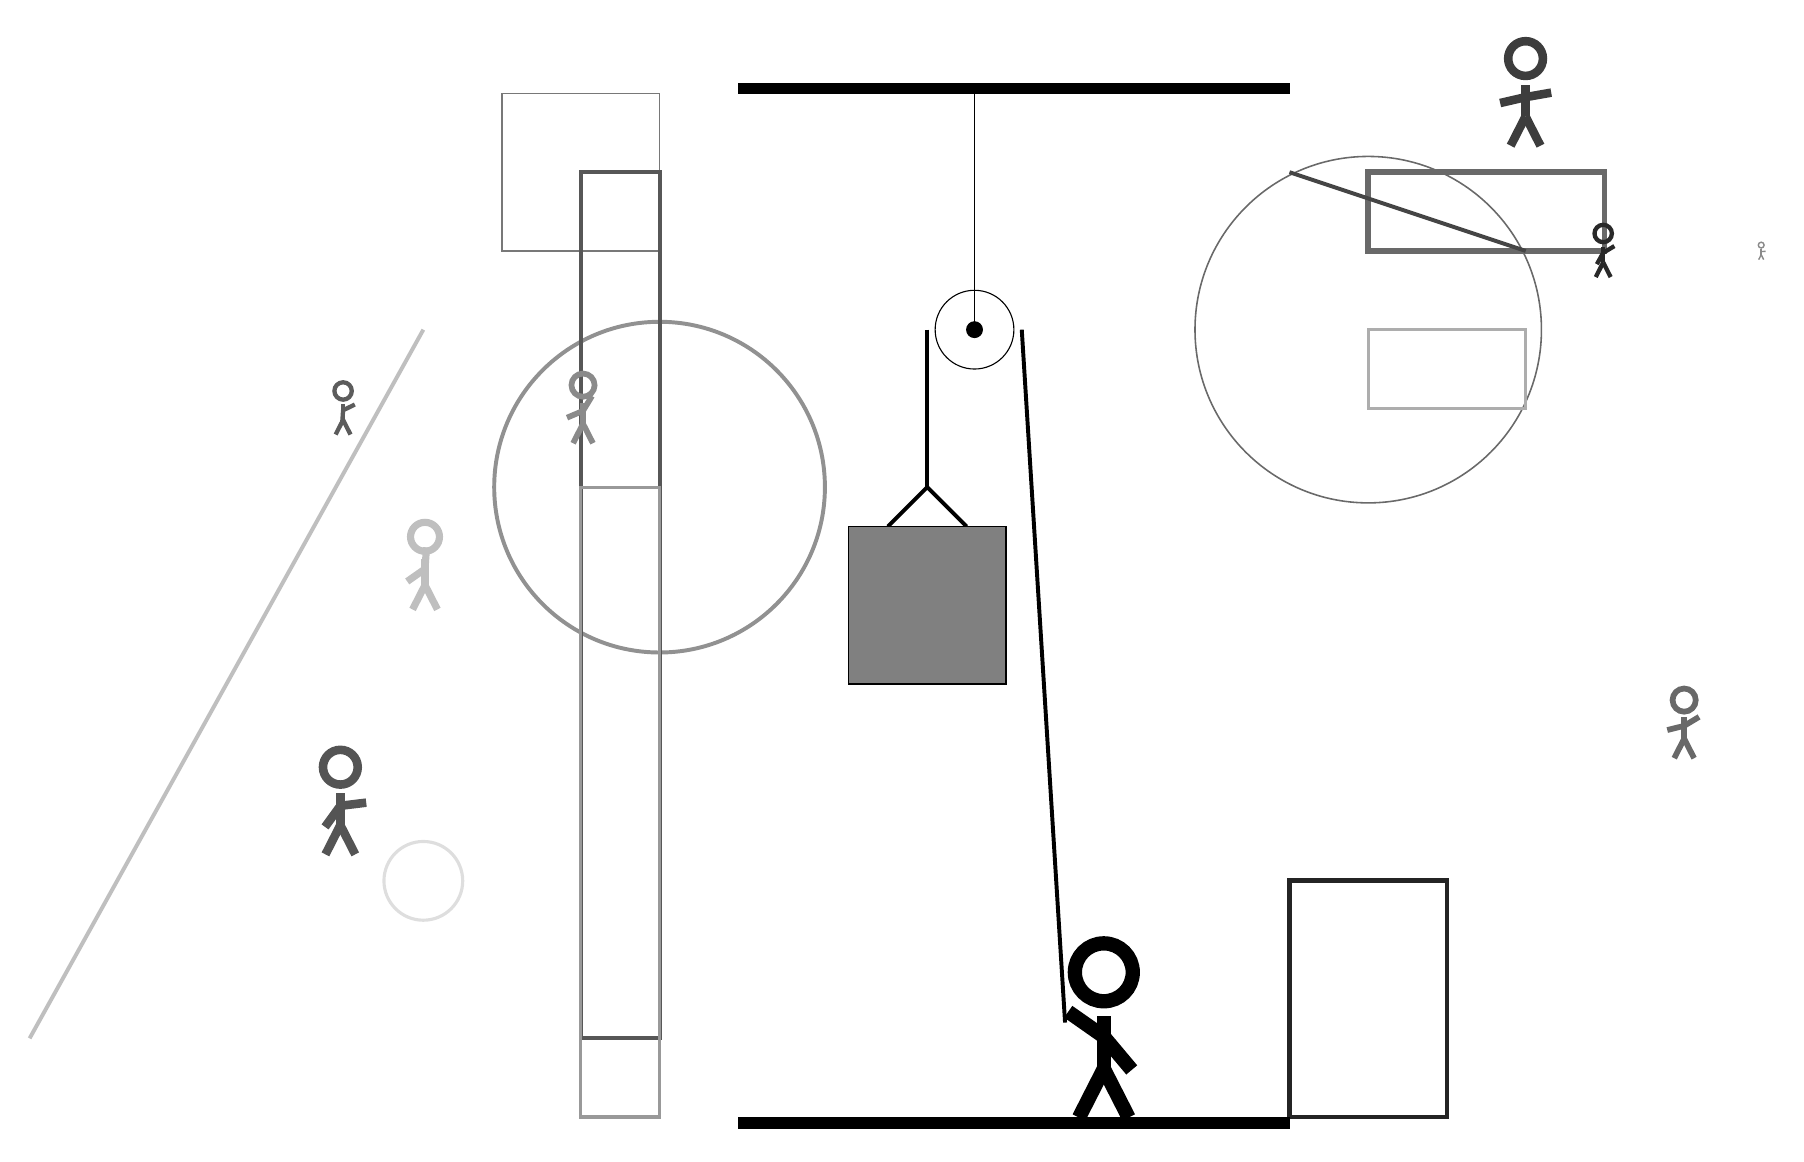
\begin{tikzpicture}
		%%%%% START %%%%%
		
		\draw[fill=black] (-2, 10) rectangle (5, 10.125);
		
		\draw (1, 7) circle (0.5);
		\draw[fill=black] (1, 7) circle (0.1);
		\draw (1, 10) -- (1, 7);
		
		\draw[line width=0.5mm] (-0.1, 4.5) -- (0.4, 5.0) -- (0.9, 4.5);
		\draw[fill=black!50] (-0.6, 4.5) rectangle (1.4, 2.5);
		
		\draw [line width=0.2mm, color=black!59](6, 7) circle (2.2);
		
		\node[line width=0.5mm, color=black!59] at (10, 2) {\Strichmaxerl[4][14][31]};
		\node[line width=0.6mm, color=black!67] at (-7, 1) {\Strichmaxerl[6][54][7]};
		\draw [line width=0.5mm, color=black!43](-3, 5) circle (2.1);
		\draw[line width=0.4mm, color=black!32] (6, 7) rectangle (8, 6);
		
		\draw [line width=0.4mm, color=black!13](-6, 0) circle (0.5);
		\node[line width=0.2mm, color=black!25] at (-6, 4) {\Strichmaxerl[5][35][86]};
		
		\draw[line width=0.7mm, color=black!59] (6, 9) rectangle (9, 8);
		\draw[line width=0.2mm, color=black!53] (-3, 10) rectangle (-5, 8);
		\node[line width=0.3mm, color=black!84] at (9, 8) {\Strichmaxerl[3][61][31]};
		
		\node[line width=0.2mm, color=black!46] at (11, 8) {\Strichmaxerl[1][83][2]};
		\draw[line width=0.5mm, color=black!73](8, 8) -- (5, 9);
		\node[line width=0.5mm, color=black!64] at (-7, 6) {\Strichmaxerl[3][86][26]};
		
		\draw[line width=0.5mm, color=black!25](-6, 7) -- (-11, -2);
		\draw[line width=0.5mm, color=black!66] (-4, -2) rectangle (-3, 9);
		\draw[line width=0.4mm, color=black!40] (-3, 5) rectangle (-4, -3);
		
		\node[line width=0.3mm, color=black!46] at (-4, 6) {\Strichmaxerl[4][23][59]};
		
		\node[line width=0.4mm, color=black!76] at (8, 10) {\Strichmaxerl[6][13][10]};
		\draw[line width=0.6mm, color=black!86] (7, -3) rectangle (5, 0);
		
		
		\draw[line width=0.5mm] (0.4, 7) -- (0.4, 5.0);
		\centerarc[line width=0.5mm](1, 7)(0:180:0.6);
		\draw[line width=0.5mm](1.6, 7) -- (2.15, -1.8);
		
		\node at (2.6, -1.9) {\Strichmaxerl[10][-35][-50]};
		
		\draw[fill=black] (-2, -3) rectangle (5, -3.15);
		
		%%%%% END %%%%%
	\end{tikzpicture}
\end{document}